\documentclass[a4paper,12pt]{report}

\usepackage{cmap}
\usepackage[T2A]{fontenc}
\usepackage[utf8]{inputenc}
\usepackage[english,russian]{babel}
\usepackage{listings}
\usepackage{amsmath}
\usepackage{float}
\usepackage{csquotes}
\usepackage{mathtools}
\usepackage{hyphenat}
\usepackage{amsfonts}

\usepackage{xcolor}
\usepackage{hyperref}

\usepackage{graphicx}
\graphicspath{ {./images/} }

\definecolor{dkgreen}{rgb}{0,0.6,0}
\definecolor{gray}{rgb}{0.5,0.5,0.5}
\definecolor{mauve}{rgb}{0.58,0,0.82}

\lstset{
    language=Python,                 
    basicstyle=\small\sffamily, 
    numbers=left,               
    numberstyle=\tiny,           
    stepnumber=1,                   
    numbersep=5pt,                
    aboveskip=3mm,
    belowskip=3mm,
    showstringspaces=false,
    columns=flexible,
    captionpos=b, 
    basicstyle={\small\ttfamily},
    numbers=left,
    numberstyle=\tiny\color{gray},
    keywordstyle=\color{blue},
    commentstyle=\color{mauve},
    stringstyle=\color{dkgreen},
    breaklines=true,
    breakatwhitespace=true,
    tabsize=3
}

\title{Лабораторная работа №5\\Автокорреляция}
\author{Крынский Павел}
\date{\today}

\begin{document}

\maketitle
\tableofcontents
\listoffigures
\lstlistoflistings

\maketitle

\chapter{Упражнение 5.1}

Я позаимствовал запись вокального чирпа, который использовался выше.

\begin{lstlisting}[caption=Вокальный чирп]
wave = thinkdsp.read_wave('28042__bcjordan__voicedownbew.wav')
wave.normalize()
wave.make_audio()
\end{lstlisting}

Далее я взял сегмент, который начинается с 0.3 секунды после начала и длительностью 0.01 секунды:

\begin{lstlisting}[caption=Первый сегмент]
sg = wave.segment(start = 0.2 , duration = 0.01)
\end{lstlisting}

Применим автокорреляционную функцию, чтобы оценить высоту тона:

\begin{lstlisting}[caption=Оценка высоты тона]
lags, corrs = autocorr(sg)
thinkplot.plot(lags, corrs)
thinkdsp.decorate(xlabel='Lag(index)',ylabel='Correlation')
\end{lstlisting}

\begin{figure}[H]
        \centering
        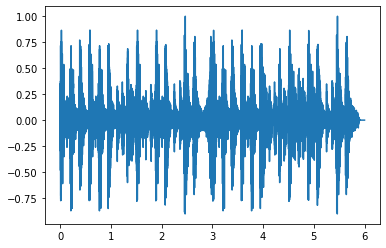
\includegraphics[width=0.75\textwidth]{1.png}
        \caption{Высота тона}
        \label{fig:lab5_fig1_1}
\end{figure}

Пик находится между 100 и 150. Используем \texttt{argmax}, чтобы уточнить значение \texttt{lag} для этого пика:

\begin{lstlisting}[caption=Нахождение \texttt{lag}]
lag = np.array(corrs[100:150]).argmax() + 100
lag
\end{lstlisting}

Находим соответствующую частоту для \texttt{lag} = 109:

\begin{lstlisting}[caption=Нахождение частоты]
p = lag / sg.framerate
fr = 1/p
fr
\end{lstlisting}

Частота равняется \texttt{436.63366336633663}.

Теперь рассмотрим сегмент сигнала через 1 секунду и проделаем аналогичные действия.

\begin{lstlisting}[caption=Второй сегмент]
sg = wave.segment(start = 1 , duration = 0.01)
\end{lstlisting}

Применим автокорреляционную функцию, чтобы оценить высоту тона:

\begin{lstlisting}[caption=Оценка высоты тона]
lags, corrs = autocorr(sg)
thinkplot.plot(lags, corrs)
thinkdsp.decorate(xlabel='Lag(index)',ylabel='Correlation')
\end{lstlisting}

\begin{figure}[H]
        \centering
        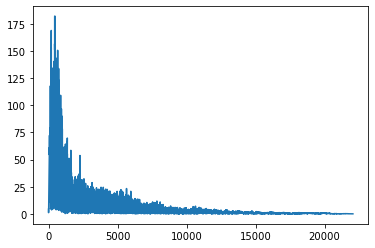
\includegraphics[width=0.75\textwidth]{2.png}
        \caption{Высота тона}
        \label{fig:lab5_fig1_2}
\end{figure}

Пик снова находится между 100 и 150. Используем \texttt{argmax}, чтобы уточнить значение \texttt{lag} для этого пика:

\begin{lstlisting}[caption=Нахождение \texttt{lag}]
lag = np.array(corrs[100:150]).argmax() + 100
lag
\end{lstlisting}

Находим соответствующую частоту для \texttt{lag} = 134:

\begin{lstlisting}[caption=Нахождение частоты]
p = lag / sg.framerate
fr = 1/p
fr
\end{lstlisting}

Частота равняется \texttt{329.1044776119403}. Отсюда можно сделать вывод, что основная частота ожидаемо уменьшается при увеличении времени начала сегмента.

\chapter{Упражнение 5.2}

Загрузим тот же вокальный чирп.

\begin{lstlisting}[caption=Загрузка звука]
wave = thinkdsp.read_wave('28042__bcjordan__voicedownbew.wav')
wave.normalize()
wave.make_audio()
\end{lstlisting}

Воспользуемся примером кода из \texttt{chap05.ipynb}. Вот его спектрограмма:

\begin{lstlisting}[caption=Спектрограмма звука]
wave.make_spectrogram(2048).plot(high=4200)
thinkdsp.decorate(xlabel='Time (s)',ylabel='Frequency (Hz)')
\end{lstlisting}

\begin{figure}[H]
        \centering
        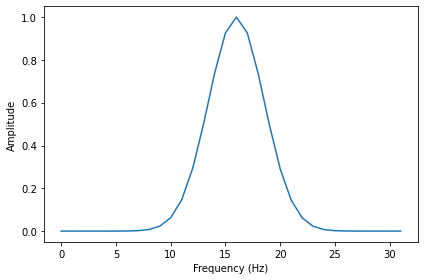
\includegraphics[width=0.75\textwidth]{3.png}
        \caption{Сегменты звуков}
        \label{fig:lab5_fig2_1}
\end{figure}

Инкапсулируем предлагаемый код в функцию. Найти первый самый высокий пик в автокорреляционной функции сложно. Поэтому мы просто укажем диапазон \texttt{lag} для поиска.

\begin{lstlisting}[caption=Инкапсуляция функции]
def estimate_fundamental(segment, low=70, high=150):
    lags, corrs = autocorr(segment)
    lag = np.array(corrs[low:high]).argmax() + low
    period = lag / segment.framerate
    frequency = 1 / period
    return frequency
\end{lstlisting}

Рассмотрим пример работы функции:

\begin{lstlisting}[caption=Пример работы функции]
duration = 0.01
segment = wave.segment(start=0.2, duration=duration)
freq = estimate_fundamental(segment)
freq
\end{lstlisting}

Результатом работы получилась частота \texttt{436.63366336633663}.

Используем написанную функцию для отслеживания высоты тона записанного звука. \texttt{ts} - средние точки каждого сегмента.

\begin{lstlisting}[caption=Отслеживание высоты тона]
step = 0.05
starts = np.arange(0.0, 1.4, step)

ts = []
freqs = []

for start in starts:
    ts.append(start + step/2)
    segment = wave.segment(start=start, duration=duration)
    freq = estimate_fundamental(segment)
    freqs.append(freq)
\end{lstlisting}

Рассмотрим кривую отслеживания высоты тона, наложенную на спектрограмму:

\begin{lstlisting}[caption=Кривая отслеживания высоты тона на спектрограмме]
wave.make_spectrogram(2048).plot(high=900)
thinkplot.plot(ts, freqs, color='blue')
thinkdsp.decorate(xlabel='Time (s)', ylabel='Frequency (Hz)')
\end{lstlisting}

\begin{figure}[H]
        \centering
        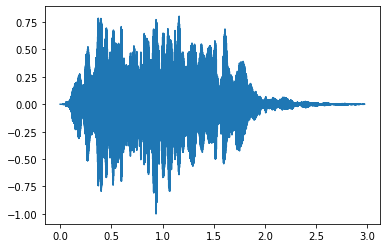
\includegraphics[width=0.75\textwidth]{4.png}
        \caption{Кривая отслеживания высоты тона на спектрограмме}
        \label{fig:lab5_fig2_2}
\end{figure}

Наложив оценки высоты тона на спектрограмму записи, можно видеть, что функция полностью справляется со своей задачей.

\chapter{Упражнение 5.3}

Воспользуемся данными о ежедневной цене \texttt{BitCoin} в течение года из прошлой лабораторной работы.

\begin{lstlisting}[caption=Таблица данных]
data = pd.read_csv('BTC_USD_2013-10-01_2021-05-22-CoinDesk.csv', parse_dates=[0])
data
\end{lstlisting}

Визуализируем скачанные данные.

\begin{lstlisting}[caption=Визуализация данных]
wave = thinkdsp.Wave(data['Closing Price (USD)'], data.index, framerate=1)
wave.plot()
thinkdsp.decorate(xlabel='Time (days)', ylabel='Price of BitCoin ($)')
\end{lstlisting}

\begin{figure}[H]
        \centering
        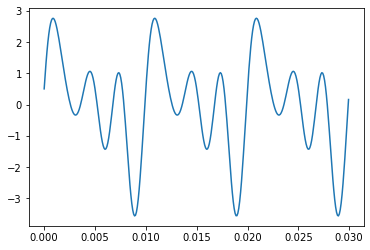
\includegraphics[width=0.75\textwidth]{5.png}
        \caption{Визуализация данных}
        \label{fig:lab5_fig3_2}
\end{figure}

Воспользуемся функцией автокорреляции, использующая статистическое определение, то есть она сдвигает среднее значение к нулю, делит на стандартное отклонение и делит сумму на N.

\begin{lstlisting}[caption=Автокорреляция при помощи \texttt{autocorr}]
from autocorr import autocorr

lags, corrs = autocorr(wave)
thinkplot.plot(lags, corrs)
thinkdsp.decorate(xlabel='Lag', ylabel='Correlation')
\end{lstlisting}

\begin{figure}[H]
        \centering
        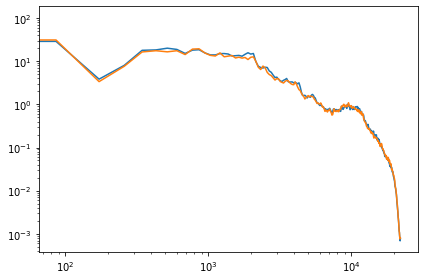
\includegraphics[width=0.75\textwidth]{6.png}
        \caption{Автокорреляция при помощи \texttt{autocorr}}
        \label{fig:lab5_fig3_3}
\end{figure}

Автокорреляционная функция падает медленно, поскольку задержка увеличивается, предполагая какой-то розовый шум.


Результат симметричен, потому что два сигнала идентичны, и отрицательный \texttt{lag} у одного даёт такой же эффект, как и положительный \texttt{lag} у другого. Вторая половина результата соответствует положительным \texttt{lag}:

\begin{lstlisting}[caption=Вторая половина результата]
N = len(wave)
corrs2 = np.correlate(wave.ys, wave.ys, mode='same')
lags = np.arange(-N//2, N//2)
thinkplot.plot(lags, corrs2)
thinkdsp.decorate(xlabel='Lag',ylabel='Dot product')
\end{lstlisting}

\begin{figure}[H]
        \centering
        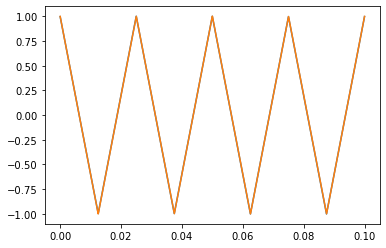
\includegraphics[width=0.75\textwidth]{7.png}
        \caption{Автокорреляция при помощи \texttt{autocorr}}
        \label{fig:lab5_fig3_4}
\end{figure}

Для этого набора данных, вероятно, более уместно статистическое определение автокорреляционной функции.

\chapter{Упражнение 5.4}

В данном упражнении я просмотрел прикрепленный ролик на YouTube и изучил все примеры, которые были приведены в файле saxophone.ipynb для разных форматов записи.

\chapter{Выводы}

Во время выполнения лабораторной работы получены навыки работы с корреляцией, последовательной корреляцей, автокорреляцей. Также рассмотрена автокорреляционная функция (АКФ).

\end{document}